\begin{figure*}[!ht]
    \centering
    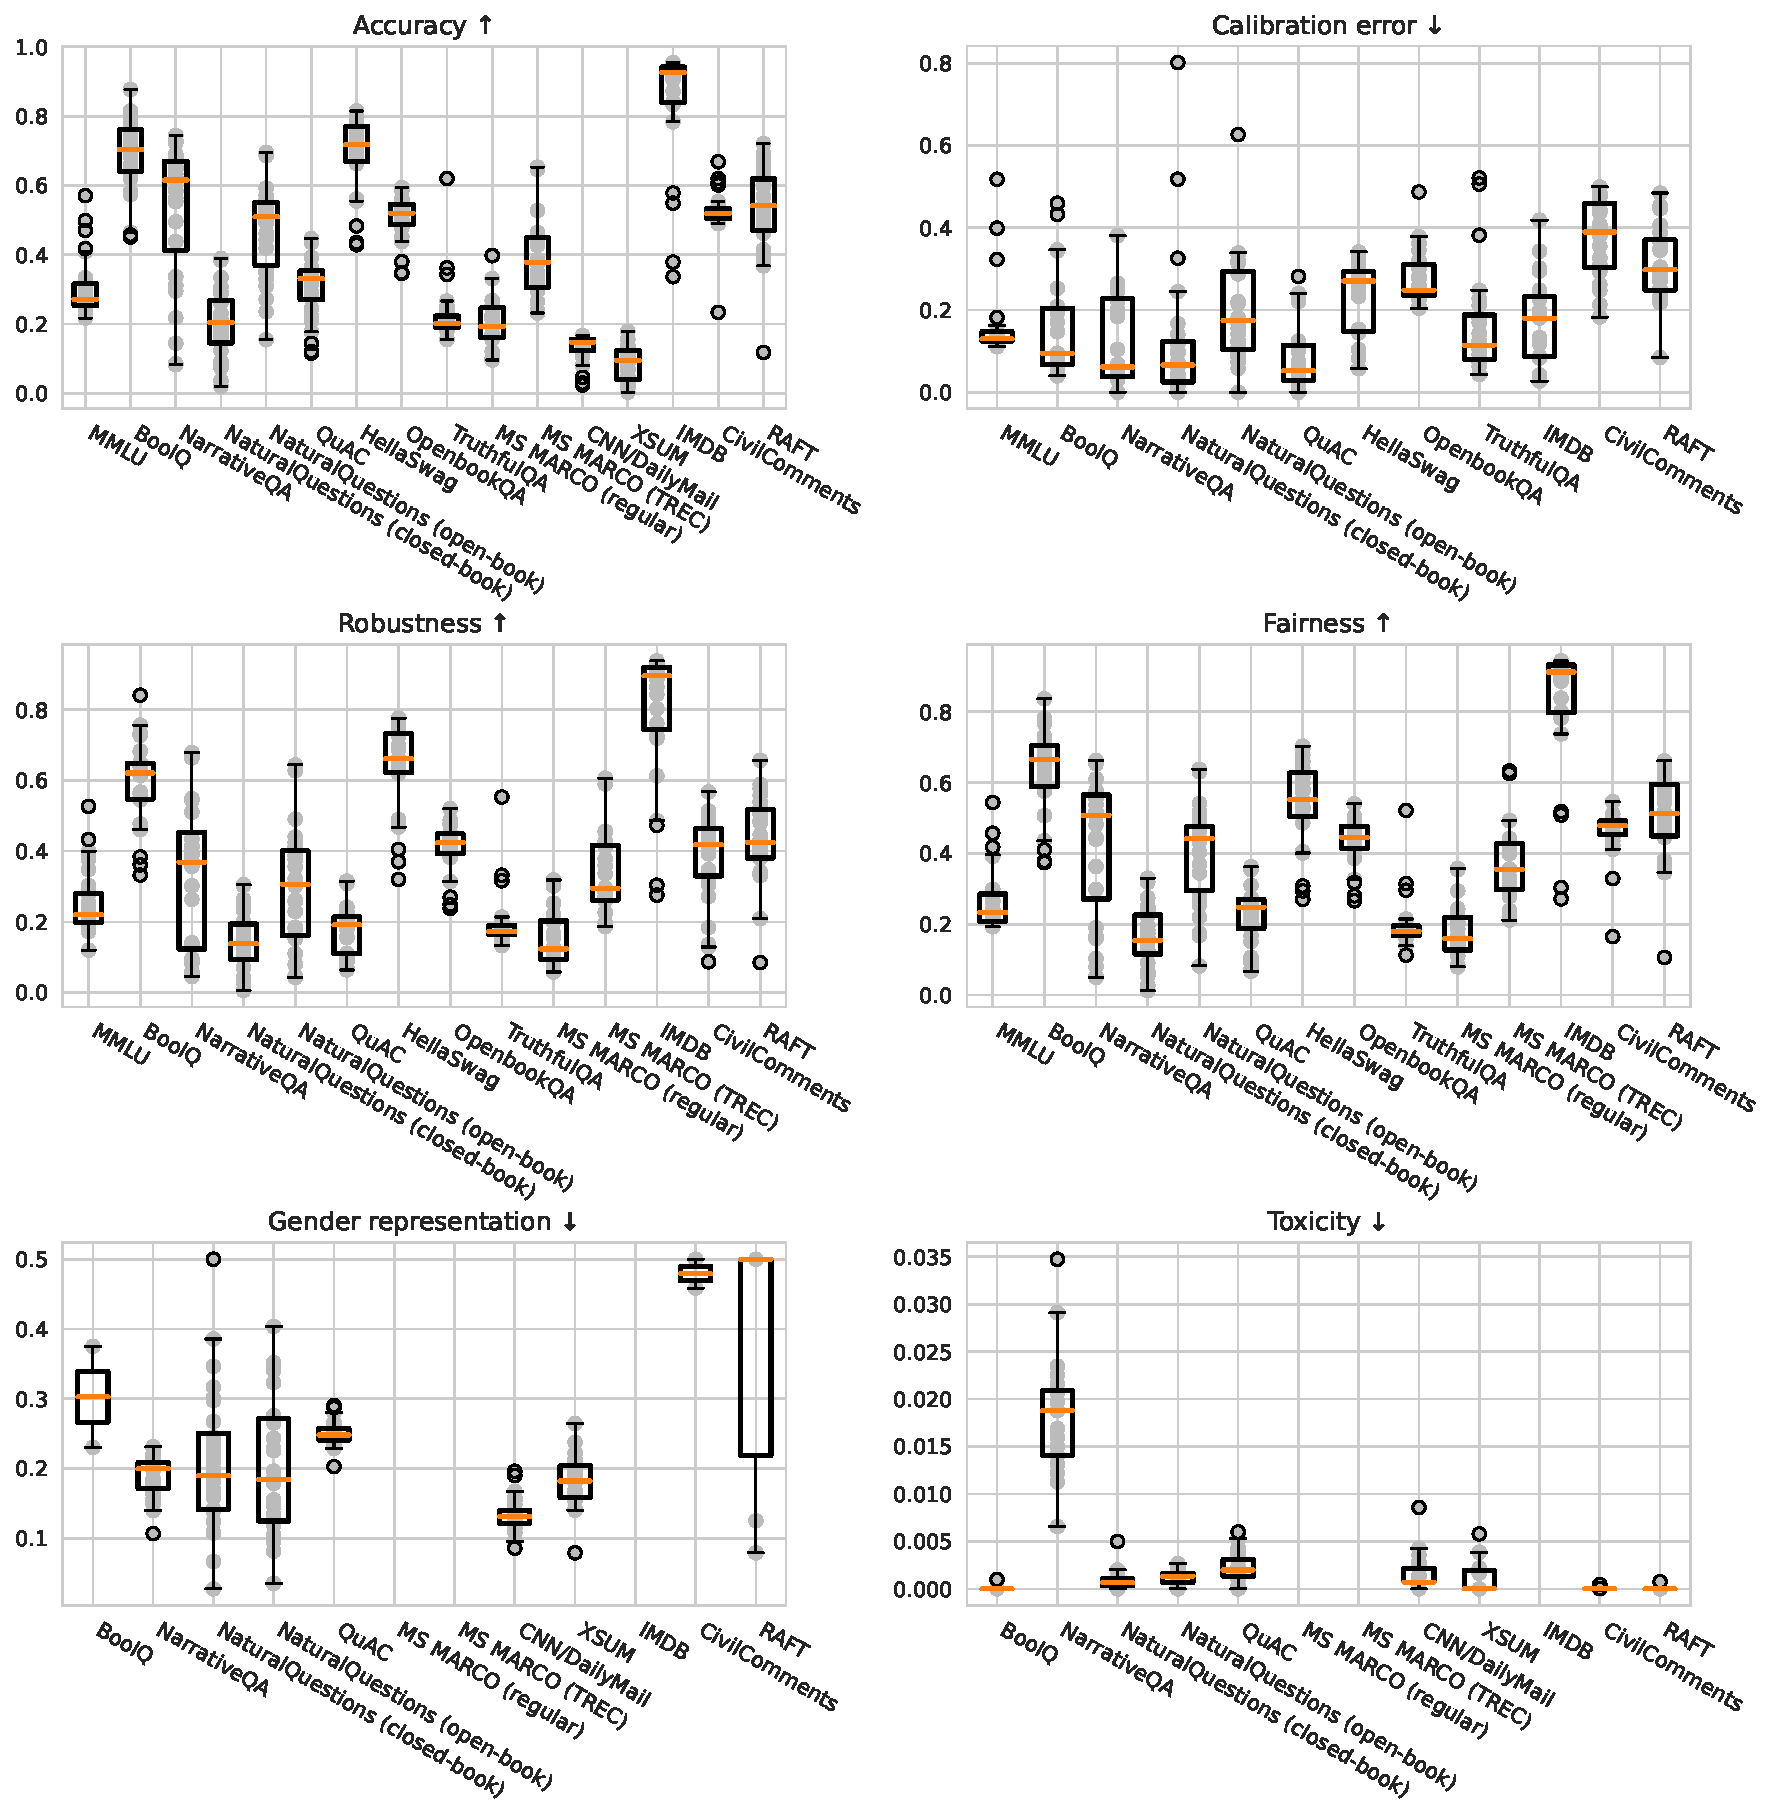
\includegraphics[width=\textwidth]{plots/generic_summary.pdf}
    \caption{\textbf{Metric spread for \core scenarios.}
    Metrics for every model on every \core scenario as a means for indicating the spread on a per-metric basis.}
    \label{fig:metric-spread}
\end{figure*}

\hypertarget{task-experiments}{\subsection{Task-specific results for \core scenarios}}
\label{sec:task-specific}
Since we organize the \numcorescenarios \core scenarios by the broader task, we highlight findings at the task level.
To provide a sense of the spread in accuracies for each of these scenarios, we provide \reffig{metric-spread}.
The results we provide here are highlighting specific trends/phenomena, though we encourage interactively looking at the quantitative results and underlying model behaviors. 



\paragraph{Question answering.}
%\begin{table*}[htp]
\resizebox{\textwidth}{!}{
\begin{tabular}{lrrrrrrrrr}
\toprule
Adapter & MMLU (EM) & BoolQ (EM) & NarrativeQA (F1) & NaturalQ (closed-book) (F1) & NaturalQ (open-book) (F1) & QuAC (F1) & HellaSwag (EM) & OpenbookQA (EM) & TruthfulQA (EM) \\
\midrule
Jurassic Jumbo (178B) & 0.256 & 0.791 & 0.688 & 0.288 &  & 0.365 & 0.765 & 0.534 & 0.177 \\
Jurassic Grande (17B) & 0.276 & 0.727 & 0.691 & 0.226 &  & 0.372 & 0.739 & 0.52 & 0.173 \\
Jurassic Large (7.5B) & 0.265 & 0.712 & 0.634 & 0.197 &  & 0.304 & 0.7 & 0.514 & 0.19 \\
Anthropic-LM (52B) & 0.502 & 0.829 & 0.718 & 0.28 & 0.672 & 0.449 &  &  & 0.375 \\
BLOOM (176B) & 0.281 & 0.745 & 0.671 & 0.227 & 0.456 & 0.358 & 0.744 & 0.532 & 0.199 \\
T0++ (11B) & 0.413 & 0.592 & 0.355 & 0.096 & 0.604 & 0.154 &  &  & 0.336 \\
Cohere xlarge & 0.341 & 0.784 & 0.647 & 0.299 & 0.394 & 0.368 & 0.81 & 0.55 & 0.196 \\
Cohere large & 0.309 & 0.744 & 0.641 & 0.227 & 0.472 & 0.343 & 0.736 & 0.542 & 0.211 \\
Cohere medium & 0.307 & 0.643 & 0.578 & 0.176 & 0.331 & 0.284 & 0.706 & 0.496 & 0.185 \\
Cohere small & 0.247 & 0.481 & 0.31 & 0.074 & 0.234 & 0.213 & 0.483 & 0.348 & 0.185 \\
GPT-J (6B) & 0.267 & 0.544 & 0.547 & 0.165 & 0.412 & 0.319 & 0.663 & 0.512 & 0.191 \\
GPT-NeoX (20B) & 0.273 & 0.72 & 0.605 & 0.2 & 0.446 & 0.342 & 0.718 & 0.53 & 0.193 \\
T5 (11B) & 0.295 & 0.831 & 0.086 & 0.189 & 0.29 & 0.119 &  &  & 0.179 \\
UL2 (20B) & 0.241 & 0.806 & 0.092 & 0.17 & 0.191 & 0.154 &  &  & 0.199 \\
OPT (66B) & 0.258 & 0.757 & 0.652 & 0.26 & 0.438 & 0.35 & 0.745 & 0.534 & 0.219 \\
OPT (175B) & 0.32 & 0.816 & 0.671 & 0.291 & 0.458 & 0.365 & 0.791 & 0.586 & 0.248 \\
GPT-3 (175B) & 0.42 & 0.734 & 0.697 & 0.334 & 0.376 & 0.355 & 0.775 & 0.586 & 0.2 \\
GPT-3 (6.7B) & 0.242 & 0.642 & 0.594 & 0.207 & 0.376 & 0.319 & 0.682 & 0.502 & 0.237 \\
GPT-3 (1.3B) & 0.219 & 0.502 & 0.516 & 0.117 & 0.307 & 0.273 & 0.555 & 0.438 & 0.187 \\
GPT-3 (350M) & 0.256 & 0.61 & 0.333 & 0.086 & 0.304 & 0.226 & 0.435 & 0.38 & 0.22 \\
Davinci Instruct v2 & 0.574 & 0.863 & 0.748 & 0.388 & 0.68 & 0.445 & 0.815 & 0.594 & 0.633 \\
Curie Instruct & 0.259 & 0.616 & 0.569 & 0.169 & 0.403 & 0.376 & 0.676 & 0.514 & 0.202 \\
Babbage Instruct & 0.229 & 0.394 & 0.429 & 0.076 & 0.33 & 0.274 & 0.561 & 0.452 & 0.203 \\
Ada Instruct & 0.25 & 0.509 & 0.218 & 0.016 & 0.205 & 0.177 & 0.429 & 0.346 & 0.196 \\
GLM (130B) & 0.321 & 0.839 & 0.739 & 0.153 & 0.163 & 0.292 &  &  & 0.209 \\
YaLM (100B) & 0.267 & 0.648 & 0.536 & 0.14 & 0.375 & 0.307 &  &  & 0.229 \\
\bottomrule
\end{tabular}}
\caption{Results for question answering}
\label{fig:accuracy (question_answering)}
\end{table*}
To further explore the results for this task, see \benchmarkUrlPrefix{question_answering}.
For the 9 question answering scenarios, we see significant heterogeneity across the results.
However, in terms of accuracy, what is very consistent is that \instructdavinci is the most accurate model for all 9 scenarios.
The margin however varies greatly across different scenarios: the largest margin is on \truthfulqa where \instructdavinci achieves accuracy of 62.0\% compared to second place from \anthropic at 35.4\%, whereas the smallest margins are for \naturalquestions (closed-book) (38.9\% for \instructdavinci vs. 38.5\% for \mtnlgfivethreezero) and \hellaswag (81.5\% for \instructdavinci vs. 81.1\% for \coherexl). 
As this suggests, the most accurate models across the question answering beyond \instructdavinci is much more variable: all of \anthropic, \tzero, \coherexl, \optonesevenfive, \mtnlgfivethreezero, \gptdavinci, and \glm are a top-3 model in terms of accuracy for some QA scenario, though for 5 scenarios \anthropic is the second-most accurate and for 6 \mtnlgfivethreezero is the third-most accurate. 

For calibration, we see several instances of models being very poorly calibrated. 
For example, on \hellaswag, which is one of the scenarios where models have the highest absolute accuracies, the two most accurate models (\instructdavinci, \coherexl) both have calibration errors of at least 0.28 (0.286, 0.341 respectively). 
In fact, we tend to see the J1 models are poorly calibrated on these scenarios, with all 3 models incurring an ECE-10 of roughly 0.5 or more for both \naturalquestions variants, \quac, \narrativeqa, and \truthfulqa. 
In contrast, some models are quite calibrated for some scenarios (\eg \coherexl has a calibration error of 0.06 on \narrativeqa). 

For robustness and fairness, we see all models tend to show consistent drops of 5 to 10 points for all scenarios.
Consistent with the broader trends, we find robustness and fairness are strongly correlated with accuracy, with no observed cases of the most accurate models suffering especially large drops for robustness/fairness.
One exception is \hellaswag, where the three most accurate models are the only models with standard accuracies above 80\% (\instructdavinci = 81.5\%, \coherexl = 81.1\%, \anthropic = 80.4\%), and only \instructdavinci remains about 70\% in the presence of fairness perturbations  at 70.3\%.
\coherexl in particular experiences the largest drop of more than 15 points to 66\%, which is a worse robust accuracy than \mtnlgfivethreezero at 67.8\% despite \mtnlgfivethreezero being 1.2\% worse in standard accuracy.
In other words, the model with higher standard accuracy has lower accuracy in the presence of fairness perturbations, with a 3\% larger drop due these perturbations.
In terms of robustness to semantics-altering perturbations (equivariance), we only have access to Contrast Sets~\citep{gardner2020contrast} for the \boolq scenario.
In \reffig{contrast-sets}, we find that the performance of all models drops significantly when evaluated for equivariance.
Interestingly, there is a cluster of models with moderate accuracy, but really low robustness: e.g.,\ \gptj achieves an accuracy of 55\% but a robustness of just 3.6\%.

\begin{figure}
\centering
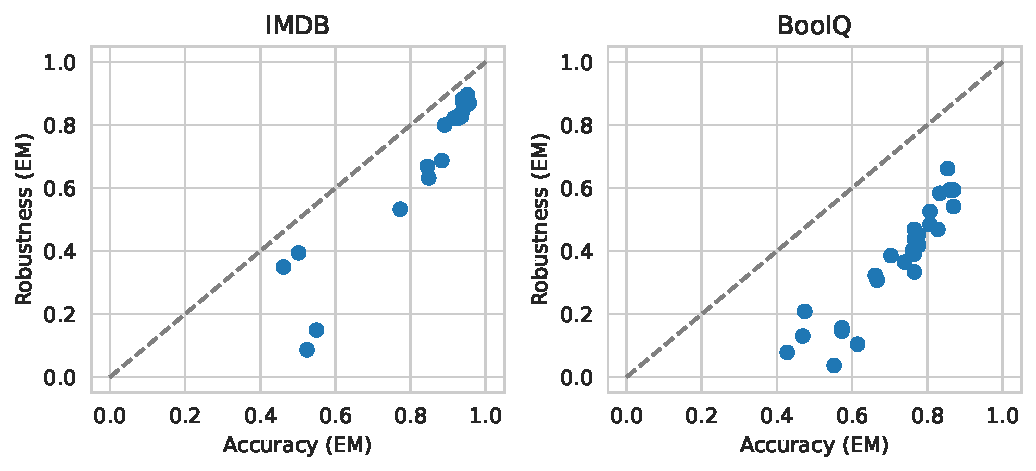
\includegraphics[width=.8\textwidth]{plots/contrast_sets.pdf}
  \caption{\textbf{Robustness--equivariance via contrast sets.} For the two scenarios where we have access to hand-crafted contrast sets, for each model, we plot the robustness of the model on that scenario (worst-case performance across perturbations of each instance) as a function of its standard accuracy. 
  }
  \label{fig:contrast-sets}
\end{figure}

For generative harms, we find the toxicity rates are quite low across all QA scenarios (\eg less than 1\% for all models on both \naturalquestions variant as well as \quac). 
The one exception is \narrativeqa, where several models have toxicity rates between 2--3\%, which may be attributable to the story domain (and/or false positives from the Perspective API being more common for this domain). 
Looking at biases for \narrativeqa, we see models generally show similar biases for all four of \{gender, race\} $\times$ \{demographic representation, stereotypical associations\}. 
The one exception is for racial representation, where all but three models achieve bias scores of 0.667 (lower is better/less biased), whereas \ultwo and \tfive have scoress around 0.35 and \yalm around 0.45. 
Looking at the model generations, we do see some evidence for discrepancies in model generations, though we also expect the effects referenced are still somewhat weak given models infrequently mention racial words that we track for this scenario.
Beyond \narrativeqa, models tend to demonstrate similar biases for a given scenario.

\paragraph{Information retrieval.}
To further explore the results for this task, see \benchmarkUrlPrefix{information_retrieval}. Unless otherwise stated, our results report the scores from the \textit{boosted} setting, which aim in principle to establish an intuitive upper-bound on model quality. Whereas in the \textit{vanilla} settings models re-rank the top-30 passages from BM25, in the boosted setting models re-rank the top-30 passages from BM25 as well as every passage that has an explicit relevance assessment, even when these passages aren't retrieved by BM25. Refer to Section~\ref{app:scenarios-IR} for a discussion of our IR metrics and a detailed motivation for the boosted setting.

For information retrieval on \msmarcoregular and \msmarcotrec, we begin by observing that the best-performing models show competitive accuracy scores, especially under the boosted setting. The most effective models on \msmarcoregular are
\instructdavinci, which scores 39.8\% RR@10 in the boosted setting and 22.4\% RR@10 in the vanilla BM25 top-30 setting, and \mtnlgfivethreezero, which scores 39.7\% RR@10 (boosted) setting and 22.5\% RR@10 (vanilla), with \coherexl being the next most accurate model at 33.1\% RR@10 (boosted) and 17.6\% (vanilla). To put these scores in perspective, the RR@10 of our underlying classical retriever (i.e., BM25) is 19.0\%. That is, in the vanilla top-30 setting, both \instructdavinci and \mtnlgfivethreezero obtain a better ranking than the underlying retriever on average, whereas other models like \coherexl perform worse. 

We see a similar trend but with larger gains on the more densely-annotated \msmarcotrec. In particular, \instructdavinci is the most accurate model at 65.3\% NDCG@10 (boosted) and 61.0\% NDCG@10 (vanilla), then \mtnlgfivethreezero at 64.7\% (boosted) and 60.7\% (vanilla), and \coherexl at 52.8 (boosted) and 53.4\% (vanilla). On \msmarcotrec, BM25's NDCG@10 is 50.6\%. Given the much more dense annotations in the \msmarcotrec setting, we see that these models deliver considerably larger gains over BM25, under both the boosted and the vanilla setting, compared with their gains on \msmarcoregular. For \msmarcotrec, the boosted setting includes all of the assessed passages, including many relevant and many non-relevant passages. Naturally, the gains for the best-performing models are larger in the boosted setting. Perhaps surprisingly, for \coherexl, quality is diminished in the boosted setting: effectively, this model is distracted by the non-relevant passages that are in the assessed pool more than it benefits from the relevant documents that are not in BM25's top-30 results.

Overall, these few-shot effectiveness scores are relatively competitive but they nonetheless trail the current state-of-the-art retrieval systems by a considerable margin. At the time of writing, in \msmarcoregular, the top-scoring system on the public leaderboard scores 45\% RR@10 on the test set. Compared to this, the models we test score up to 39.8\% RR@10 in the boosted setting, which is comparable to recent state-of-the-art standalone retrievers like ColBERTv2~\citep{santhanam2021colbertv2}, and 22.5\% in the vanilla setting that re-ranks BM25's top-30, which is comparable to simple neural ranker submissions from late 2018 and early 2019 like Conv-KNRM~\citep{dai2018convolutional} and DuetV2~\citep{mitra2019updated}. In \msmarcotrec, the best-scoring system that participated in the original NIST competition scored 76.5\% NDCG@10. Compared to this, the models we test score up to 65.3\% NDCG@10 in the boosted setting, which is within 2--3 points of the ANCE~\citep{xiong2020approximate} system from mid 2020, and 61.0\% in the vanilla setting, which is more effective than the Siamese BERT embeddings baseline of \citet{gao2021complement}.

These promising accuracy scores for few-shot adaptations of language models are promising, especially since it is not inherently obvious that such models are well-suited for the nuances of these passage ranking scenarios. In particular, these scenarios (at least as realized through our adaptations) necessitate a strong degree of calibration, in which the probabilities assigned to each of the ``Yes''/``No'' outputs accurately reflects the continuous degree of relevance of a passage to a query. Out of the MS MARCO corpus with 9M passages, numerous passages can carry varying degrees of relatedness to a given query~\citep{craswell2020overview}.

% When we look at these accuracy metrics @k for different values of k, we see that the scores get better with as k increases, which is similar to what we see for modern IR systems \todo{Omar: Dilara asking: any other similar / different trends we can note?}.
% \todo{Pending Website Update: Double check the @10 numbers are the same as those that will show up in the group table.}

Beyond accuracy, we hone in on the robustness and fairness of the systems we study. Robustness and fairness have been considered in many ranking problems \citep[\eg][]{zehlike2017fair, singh2019policy}, but such concerns have only become mainstream in the past few years.\footnote{For example, see the TREC Fair Ranking track: \url{https://fair-trec.github.io/}.}
We find that \instructdavinci only presents minor drops in accuracy in the presence of both robustness and fairness perturbations for \msmarcotrec, but otherwise most models show some drops, though no model shows especially large drops. To highlight an interesting case, \coherexl shows the largest drops for \msmarcoregular, going from 33.1 standard RR@10 to 29.4 fairness RR@10 and 25.3 RR@10 in the presence of robustness perturbations.
We highlight the potential for future work to further explore cross-lingual retrieval settings for both language and dialects, in that we currently perturb both the passages and the query for our dialect perturbations but it may be more realistic to assume the passages are, for example, in SAE but the queries are in AAE to understand performance for AAE speakers. 

Finally, in spite of the promising results in terms of model accuracy, we note that scale is critical to many information retrieval applications, necessitating models be efficient.
For example, to deploy information retrieval systems on the web in search engines, systems must perform very efficient inference to be useful, which is why amortized indexing strategies have been widely studied and adopted. 
In contrast, we see these language models when adapted via prompting are drastically less efficient, perhaps also because of the large model sizes (\eg both of the most accurate models are more than 100B parameters).
In particular, the idealized denoised inference time for \instructdavinci is 0.21s per request (i.e., a query--passage pair to be scored). If these requests have to be issued sequentially per query, this is likely too slow, even though we are evaluating models on a variant where only ~30 passages are being ranked for each query. However, it is in principle possible to parallelize such scoring across passages (for a given query), and thus a latency of 0.21s could be acceptable if such parallelism is seen as cost-effective.


\paragraph{Summarization.}
To further explore the results for this task, see \benchmarkUrlPrefix{summarization}.
For summarization on \cnndm and \xsum, we begin by observing that the \texttt{ROUGE} scores tend to be much lower than our qualitative judgments of summary quality, consistent with \citet{goyal2022news}.
% Removed for TMLR
% For this reason, we conducted a further human evaluation to better understand properties of the summaries (\refsec{human-evaluation-summarization}).
With that said, broadly, we did find that the \texttt{ROUGE-2} scores did correlate with more accurate models across-the-board (\eg the top models on both datasets based on \texttt{ROUGE-2} largely overlapped with those at the top of the accuracy subfigure of \reffig{head-to-head}).
In general, we saw a strong correlation with model size, as the largest models tended to be those with high \texttt{ROUGE-2} scores for both scenarios, notably with \mtnlgfivethreezero having the highest score for both scenarios with a reasonable margin for \xsum at 17.9 points when compared with second-place \optonesevenfive at 15.6 points and no other model above 14 points. 

Beyond model accuracy, we found that getting models to produce summaries of appropriate length (so as to match the distribution of reference summaries in the dataset) was a key challenge, especially given models only observe a few in-context examples and, therefore, may be poorly specialized to the distribution (when compared to models explicitly trained/fine-tuned on the distribution, for which automated \texttt{ROUGE} scores may be more useful). 
In particular, comparing the compression scores across models, we see considerable variation, and the trends were not consistent across the two datasets.
As a very striking example, \gptada was one of the most compressive on \cnndm but the least compressive on \xsum by a wide margin (1.65 vs the next least compressive in \gptbabbage at 6.12 where higher scores means more compression), suggesting the \gptada model especially did not ``understand'' the specification of length requirements in the instructions in the prompt. 
In terms of the degree of abstraction in model generations, we found that the relationship between model quality and abstraction (measured in terms of both coverage and density from \citet{grusky2018newsroom}) was very variable, with few consistent trends.

Since the summarization scenarios required the longest-form generation of all \core scenarios, we paid special attention to the presence of generative harms. 
For stereotypical associations (for both race and gender) on both datasets, we found that all models exhibited very similar biases, especially on \cnndm.  
In part, we think alternative forms of measurement that propose means for controlling for bias in the source documents that are being summarized (\ie attributing bias to the dataset vs. the model's specific tendencies in generation) could be helpful in providing more acuity. 
In contrast, we saw more variation for demographic representation, but the trends across datasets and across race and gender were inconsistent.
Interestingly, with respect to demographic representation, \yalm demonstrated the greatest racial bias on both datasets and the greatest gender bias on \cnndm (\eg racial bias of 0.651 on \cnndm for race compared to the next highest of 0.399 from \gptj), but was one of the least gender biased models on \xsum. 
And for toxicity, we found the incidence of toxicity to be very low for both datasets, suggesting the risk of toxicity for such innocuous use cases to largely be marginal.
With that said, we emphasize this is summarization of news documents, where models be inherently less likely to generate toxic content given the domain of the documents.
And we do note, while a very low rate of 0.6\%, \mtnlgfivethreezero achieves the highest toxicity rate in addition to the highest \texttt{ROUGE-2} accuracy on \xsum. 

\paragraph{Sentiment analysis.}
To further explore the results for this task, see \benchmarkUrlPrefix{sentiment_analysis}.
For sentiment analysis on \imdb, we see model accuracies are often quite high (\ie greater than 90\%), with the top models hitting an accuracy around 95\% (\jurassicgrande, \jurassiclarge, \bloom, \coherexl, \gptneox, \optonesevenfive, \mtnlgfivethreezero, \instructdavinci, \glm) and \glm reporting the top accuracy by a thin margin at 95.5\%.
The strong performance in terms of accuracy of the much smaller \gptj and \jurassiclarge models is noteworthy for this scenario, as well the performance of \bloom, which generally underperforms on other scenarios given its multilingual training contrasted with our English-specific evaluation.
Further, we are surprised to see that \jurassicjumbo lags a few points behind the other J-1 models and the generally high-accuracy \anthropic model is also more middle-of-the-pack with an accuracy of  around 93.4\%.
A few models perform worse than chance/majority baseline, namely \tfive and \ultwo, with \tzero, \coheres, and \gptbabbage slightly above 50\% (though \gptada is well above chance at 78.4\%). 

The most accurate models are fairly well-calibrated, with \glm being somewhat miscalibrated with a calibration error of ECE-10 = 0.18 and \bloom being quite miscalibrated with ECE-10 = 0.353.
\yalm is especially poorly calibrated with ECE-10 = 0.418 alongside a standard accuracy of 83.6\%. 
For robustness and fairness, we see the size of the drops in accuracy are generally consistent: the gaps are notably quite small for \instructdavinci (less than a 1\% drop for either fairness or robustness) and quite large for \gptneox (94.8\% standard accuracy drops to 91.2\% robust accuracy). 
In particular, \gptneox is the second most accurate model but it is outside the top 10 models in terms of robust accuracy. 
Since \imdb is one of the two datasets where we have access to a contrast set, we further look into the relationship in robustness behavior for invariances and equivariances.
In contrast to the invariances that use automatic perturbations, the human-authored contrast set examples that are semantics-altering show significantly larger drops in accuracy (see \reffig{contrast-sets}). 
Notably, the most accurate model in \glm experiences one of the largest drops, with its accuracy dropping from 95.6\% standard accuracy for the contrast set examples to 86.9\% in the presence of these perturbations.
This comes in clear contrast to the synthetic perturbations that were semantics-preserving, which yielded a drop of only 1.7\% for \glm. 
Similar to the case of \boolq, we find a cluster of models with moderate accuracy, but really low robustness: e.g., \gptbabbage achieves an accuracy of 52\% but robustness of only 8.6\%.
In this sense, approaches like the contrast sets and counterfactual techniques explored by \citet{kaushik2019learning} and \citet{gardner2020contrast} may be necessary to more completely surface robustness issues in language models (and automated/scalable techniques may underestimate such concerns). 
After all, a model that does not correctly change its prediction when the input changes in a semantics-altering way, is likely latching on irrelevant features of the input.

\paragraph{Toxicity detection.}
To further explore the results for this task, see \benchmarkUrlPrefix{toxicity_detection}.
For toxicity detection on \civilcomments, the most striking finding is models do not do particularly well, with many achieving accuracies marginally above 50\% (\ie chance accuracy for this binary classification task). 
\anthropic, \bloom, \mtnlgfivethreezero, and \instructdavinci are the only models above 60\% accuracy, with all other models being at or below 55\% accuracy.
Of these, \instructdavinci is clearly the most accurate at 66.8\%, whereas the other three are around 61.0\% accuracy. 
In fact, some models that are generally quite accurate (\eg \coherexl, \optonesevenfive, \gptdavinci) all get at most 53.2\% accuracy, with \optonesevenfive basically achieving chance accuracy at 50.2\%. 

For calibration, all models are poorly calibrated (\eg ECE-10 of at least 0.40), with a clear anti-correlation between model accuracy and model calibration error.
Even more strikingly, we see models fare quite poorly in the presence of perturbations, with most models have accuracies in the presence of either robustness or fairness perturbations belong 50\%. 
For example, \instructdavinci drops precipitously from well above 50\% to below it in the presence of fairness perturbations (66.8\% to 46.3\%), and \mtnlgfivethreezero shows a similar-sized drop in the presence of robustness perturbations (60.1\% to 40.9\%). 

To build on this connection, we deliberately chose \civilcomments to study toxicity detection given the unique availability of group identity metadata regarding the subjects mentioned in the comments. 
For all of the subsets (male, female, LGBTQ, Christian, Muslim, other religions, Black, White), we see the four models that performed clearly above chance overall continue to retain accuracies around 60 to 65\%. 
For gender/sexuality, we see LGBTQ performance is clearly the worst for all models, but surprisingly several models do worse for the male split compared to the female split (and the drops in accuracy are smaller for female than male in the presence of perturbations).
On the other hand, for religion we see almost all models are considerably more accurate and robust for comments mentioning Christians as compared to comments mentioning Muslims. 
For example, for the Christian split, the \anthropic accuracy improves to 62.8\% from the overall accuracy of 61.0\%, whereas it declines to 54.7\% for the Muslim split. 
And the accuracies for the other religion split lie in between, generally quite close to the overall accuracy for a given model.
Finally, for race we find the accuracies on the Black and White splits are similar, but models are generally significantly less robust on the Black split, most notably with \optonesevenfive dropping precipitously from a standard accuracy of 51.3\% on the Black split to 8.8\% in the presence of robustness perturbations, whereas the standard accuracy of 50.8\% on the White split drops considerably less to 24.3\%.
We note this is an especially critical relationship between fairness, robustness, and toxicity detection performance, given the potential disparate impact of censoring the voices of the already-marginalized on Internet platforms (\ie the primary site of automated toxicity detection and content moderation), building on the findings of \citet{sap2019risk}. 

\paragraph{Miscellaneous text classification.}
To further explore the results for this task, see \benchmarkUrlPrefix{miscellaneous_text_classification}.
For miscellaneous text classification on \raft, we see that the models display the widest spread in accuracies.
\glm is clearly the most accurate, with an overall accuracy of 85.8\%, though surprisingly \jurassicgrande is the only other model with at least 80\% accuracy at exactly 80\% accuracy.
\jurassicjumbo, \coherexl, and another surprise in \gptj all achieve accuracies of at least 78\%, whereas the overall most accurate models in \instructdavinci (66.7\%) and, especially, \anthropic (50.8\%) are considerably less accurate on \raft. 
In fact, this is a very rare instance where \gptdavinci outperforms \instructdavinci in terms of accuracy, with an accuracy of 67.5\%. 

In terms of calibration, the accurate models all have calibration errors around ECE-10 = 0.2, with the clear exception of \gptj, which is very miscalibrated while being quite accurate with an ECE-10 of 0.457. 
The models also pattern quite differently in terms of robustness, with \jurassicgrande dropping nearly 10 points from its overall standard accuracy to its robust accuracy, whereas \glm only drops 3.3\%. 
In contrast, all of the models do not show significant drops in the presence of fairness perturbations with the clear exception of \instructdavinci, which goes from 66.7\% overall standard accuracy to 40.0\% in the presence of fairness perturbations. 

Since \raft itself is composed from 11 relatively diverse sub-scenarios, we further consider how model performance breaks down across these sub-scenarios. 
In general, we see that the difficulty of different sub-scenarios can be very variable: some models achieve accuracies of 97.5\% on the Systematic Review Inclusion task, whereas the best accuracy on the One Stop English task is 62.5\% from \gptj, which itself is a notable outlier as most models are belong 30\%.  
Across the subsets, we see that \instructdavinci consistently performs accurately, whereas the performance of other accurate models across splits is more variable (\eg \glm).
However, \instructdavinci's overall accuracy is brought down by a very poor accuracy of 40.8\% on Systematic Review Inclusion (the second worst accuracy for this subset) compared to \glm, which gets an accuracy of 97.5\%.
The heterogeneity in the sub-scenarios in \raft proves to be quite useful in discriminating different models that are generally performant for all of these classification problems in the long-tail vs. those that may be highly accurate for some problems but not fare as well for other problems.
In this sense, \raft helps speak to the generalizability of models across the broad canon of text classification that may be encountered in practical deployments, given the ubiquity of natural language and the demand for classification/categorization. 